\documentclass[12pt]{article}
\usepackage{amsmath}
\usepackage{amssymb}
\usepackage{amsthm}
\usepackage{color}
\usepackage{graphicx}
\usepackage{natbib}
\usepackage{xspace}
\linespread{1.7}

\newcommand{\sdgphi}{\ensuremath{\sigma_{g\phi}}\xspace}
\newcommand{\sdphi}{\ensuremath{\sigma_{\phi}}\xspace}
\newcommand{\sdmu}{\ensuremath{\sigma_{\mu}}\xspace}
\newcommand{\dnorm}{\ensuremath{\mathbf{\Phi}}}{\xspace}

\begin{document}
Note: all parameters, including $\phi, g$, are on $\log$ scale.\\

Suppose that $\phi_{ij}$ follows a normal distribution with mean $\phi_i$ and standard deviation $\sdphi$: $\phi_{ij} \sim N(\phi_i, \sdphi^2)$, and $\phi_i$'s are i.i.d. from $N(\mu,\sdmu^2)$, where $1 \le i \le n$ and $1 \le j \le m$. (In our case, $n = 106$ and $m = 3$.) 
Suppose there is a linear relationship between $g$ and $\phi$ that holds for every gene: $g_i = a + b\phi_i$, then it follows that $g_i+\phi_i = a + (b+1)\phi_i + \epsilon_i$, for $1 \le i \le n$ where $\epsilon_i$ is the noise in the estimators/observations for gene $i$, and $\epsilon_i \sim N(0, \sdgphi^2)$. Based on these assumptions we have the probability of observing $g\phi_i$ and $\phi_{ij}$:
\begin{eqnarray}
& &P(g\phi_i, \phi_{ij} | \mu, \sdphi,\sdmu,\sdgphi,a,b)\nonumber \\ 
&=& \int P(g_i + \phi_i | a, b, \phi_i, \sdgphi)P(\phi_{ij}, \phi_i | \mu, \sdmu)\; \mathrm{d}F(\phi_i) \nonumber\\
&=& \int_{-\infty}^{\infty} \dnorm(\phi_{ij} | \phi_i,\sdphi) \dnorm(\phi_i | \mu, \sdmu) \dnorm(g_i + \phi_i | a+(b+1)\phi_i, \sdgphi)\; \mathrm{d}\phi_i \nonumber
\end{eqnarray}
�
where $\dnorm(x | \mu, \sigma)$ is the probability density function for normal distribution with mean $\mu$ and variance $\sigma^2$. 
%Here if $\sdphi$ and $\sdmu$ are switched, the probability will stay the same, and the variance of $\phi_{ij}$'s is roughly $\sdmu^2 + \sdphi^2$. 
With the likelihood function for the 6 parameters, and the observed $g_i + \phi_i$ and $\phi_{ij}$ we can find the MLE(maximum likelihood estimates) for the parameters. 

Following is a simulation with parameters $\mu = -2.7$, $a = 3$, $b = 1$, $\sdmu= 0.1$, $\sdphi = 1$ (bigger noise in the estimates of $g\phi$), $\sdgphi = 0.1$, and the following plot is produced:
\begin{figure}[h]
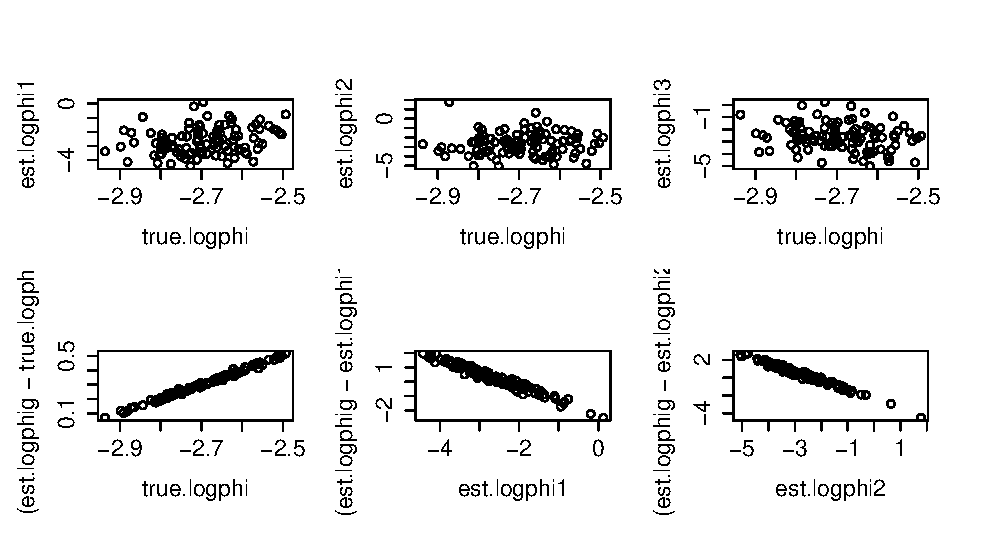
\includegraphics[width=\textwidth]{gphi.eps}
\caption{Top row: scatterplots of estimated and true values of $\log{(\phi)}$; Bottom row: scatterplots of $g$ and $\phi$.}
\label{fig:gphi}
\end{figure}
Figure \ref{fig:gphi} shows that, even though the true relationship between $g$ and $\phi$ is $g=\phi + 3$, which is linear function with positive slope, the relationship shown by the estimated data with noise is negatively correlated, exactly opposite of what is used in the simulation. Whereas the ML estimates for the parameters are not consistent with the true parameters, in that likelihood of true parameters is much smaller than that of some other parameters far from it. Possible reason for this is the impreciseness of the integral in the likelihood function caused by product of very small numbers. - results from R and Mathematica are substantially different.

Explanation of why this happens: Because of the large noise in the estimated values of $\log(\phi)$, the line describing the true relationship between $g$ and $\log(\phi)$ is going to be a line with positive slope but very big width (very thick line with positive slope). When the thickness exceeds the length of the line itself (which depends on the range of the $g$ and $\log(\phi)$), this line will look like that it has a negative slope. As the noise increases to a point when the width of the line is much bigger than the length of the line, it looks like a thin line with a negative slope.In this case, $\log(\phi g) - \log(\phi)$ is very close to $-\log(\phi) + \text{constant}$ because of small variance in $\log(\phi g)$, therefore the slope of $-1$ in the figure. 

\end{document}